\chapter{The Baseline Chipa System}
\label{chap:baseline}
Here we describe the baseline version of the Chipa software and evaluate its
performance on the tasks described in the previous chapter.
At its core, the Chipa software takes in a word-aligned bitext corpus, with
annotations for the source tokens. It then trains CL-WSD classifiers for
source-language word types on demand. 

By default, the software holds all of the available bitext in memory, or
optionally on disk, when training from larger corpora. On request, it
constructs a training set for learning to disambiguate a particular lemma
by retrieving all sentences that contain the lemma,
finding the instances of that lemma and its aligned translations, and extracting
features (see Figure~\ref{fig:baselinefeatures}) from the source sentence's
surface text and annotations.
If a source-language lemma has been seen aligned to only one target-language
type, then this is simply noted, and if the lemma is not present in the
training data, then it is marked as out-of-vocabulary. This situation will not
arise in our \emph{in vitro} evaluation, but during \emph{in vivo} machine
translation, OOV words will occur in practice.
In either of these cases, we do not train a classifier for that lemma, since
there is no ambiguity present in our examples and the Chipa software cannot
provide any useful guidance to its caller. A machine translation system may,
for example, refuse to translate sentences with OOV words, or more likely, will
simply assume the identity translation, effectively passing them through
untranslated.

Since source-language tokens may be NULL-aligned (i.e., not all words in the
source text will have corresponding words in the target text), both in the
training data and in translations, Chipa provides the option to request
classifiers that consider NULL as a valid label for classification, or not, as
appropriate for the translation application. For example, function words found
in one language may not need to have a surface representation in
the target text\footnote{As one concrete example, the Spanish ``personal
\emph{a}" typically gets no translation in any of the other languages addressed
in this work. Spanish syntax requires \emph{a} before the object of a verb,
but only when that object is a human being or (controversially) a beloved
animal.}.
We here report classification accuracies for both settings.

Memory permitting, Chipa classifiers are kept cached for later usage. Chipa can
also be run as a server, providing an interface whereby client programs can
request CL-WSD decisions over remote procedure calls (RPC).

Chipa's classifiers are trained with the scikit-learn machine learning toolkit
\cite{scikit-learn} for Python and its associated NLTK interface, though in
earlier versions, we used the megam package \cite{daume04cg-bfgs}, also through
NLTK. By default, we use Logistic Regression classifiers (also known as
Maximum Entropy), with the default scikit-learn settings.
Maximum entropy classifiers are well-suited to this sort of classification
task, as they are robust to adding large numbers of features, even
highly-correlated ones \cite{nigam1999using}. Here we have exactly this
situation, large numbers of sparse features, where some of them are likely to
be highly correlated, since our features contain several representations of the
tokens from the input sentence -- their surface forms and their lemmatized
forms, and the presence of a word in the window surrounding the focus word
guarantees its presence in the bag of words representing the entire sentence.
This is fairly typical of text classification problems.

\begin{figure*}
  \begin{centering}
  \begin{tabular}{|r|p{11cm}|}
    \hline
    name          & description  \\
    \hline
    \texttt{bagofwords}    & a feature counting each lemma in the source sentence \\
    \hline
    \texttt{bagofsurface}  & like \texttt{bagofwords}, but with surface forms \\
    \hline
    \texttt{window}       & a binary feature for each of the lemmas in the immediately surrounding three-word context window \\
    \hline
    \texttt{surfacewindow} & like \texttt{window}, but with surface forms \\
    \hline
  \end{tabular}
  \end{centering}
  \caption{Features for the baseline Chipa system}
  \label{fig:baselinefeatures}
\end{figure*}

Because we have a large number of features but a relatively small
number of samples per classifier, the literature would encourage us to train
with L1 regularization rather than L2 \cite{ng2004feature}, but we found that
the results are consistently slightly better when using L2. We could also
search for an optimal regularization hyperparameter -- the number that controls
the tradeoff between simple solutions and ones that closely fit the input,
perhaps at the risk of overfitting. We did try a few different values for the
regularization parameter, but found that the results were not dramatically
different; furthermore, we do not want to overfit our corpus by tuning
parameters too much after running tests. Here we will keep the default
regularization setting of $C=1.0$.

We have also tried a variety of classification algorithms; scikit-learn makes
experimentation with different classifiers and parameter settings
straightforward. In particular, we tried random forests and linear support
vector machines, as well as the familiar ``most frequent sense" baseline. For
the baseline feature set, for the most part we see the the best performance
from the logistic regression classifiers with L2 normalization, although the
differences are not large; the other classification algorithms that we tried in
these experiments did nearly as well.

\section{Classification Results for the Baseline System}

\begin{figure}
  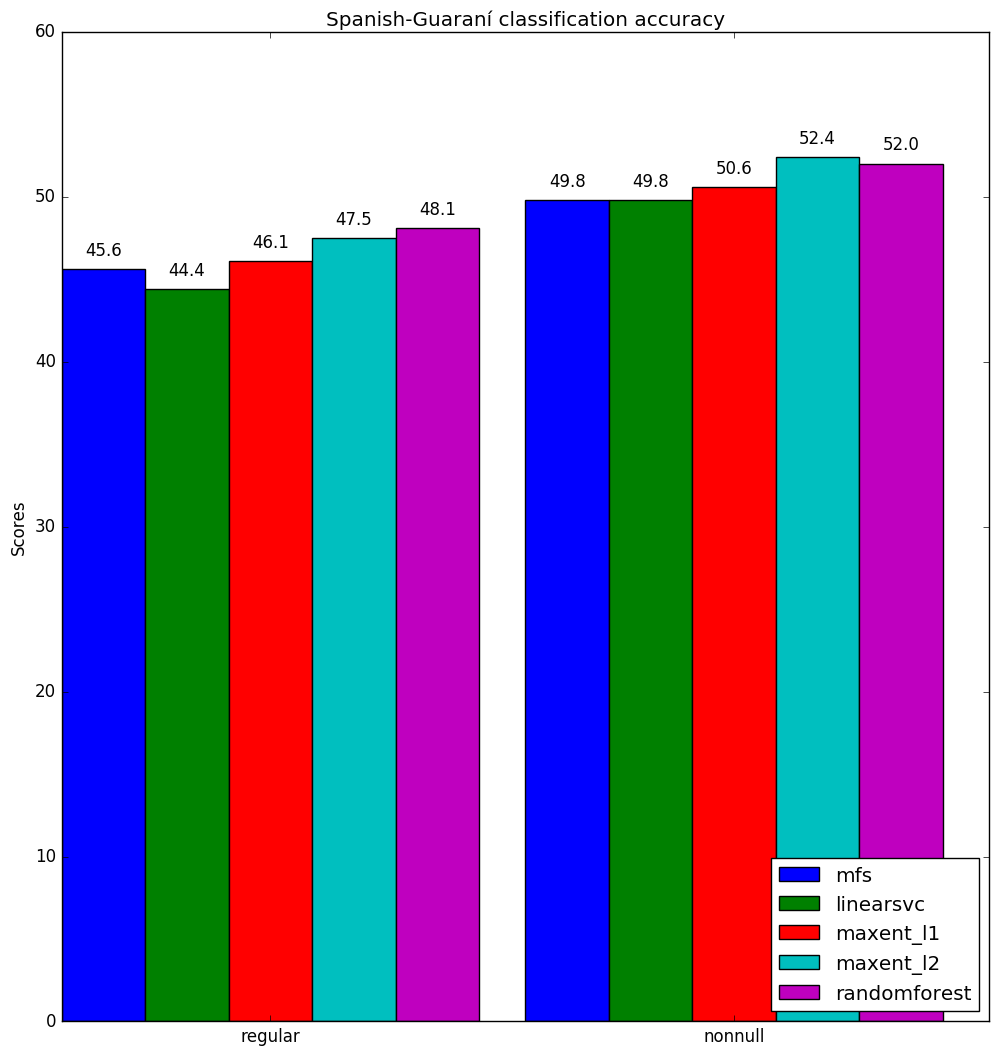
\includegraphics[width=\textwidth]{results-baseline-es-gn.png}
  \caption{Baseline Chipa scores for Spanish-Guarani, by classifier.}
  \label{fig:esgnresults:baseline}
\end{figure}

\begin{figure}
  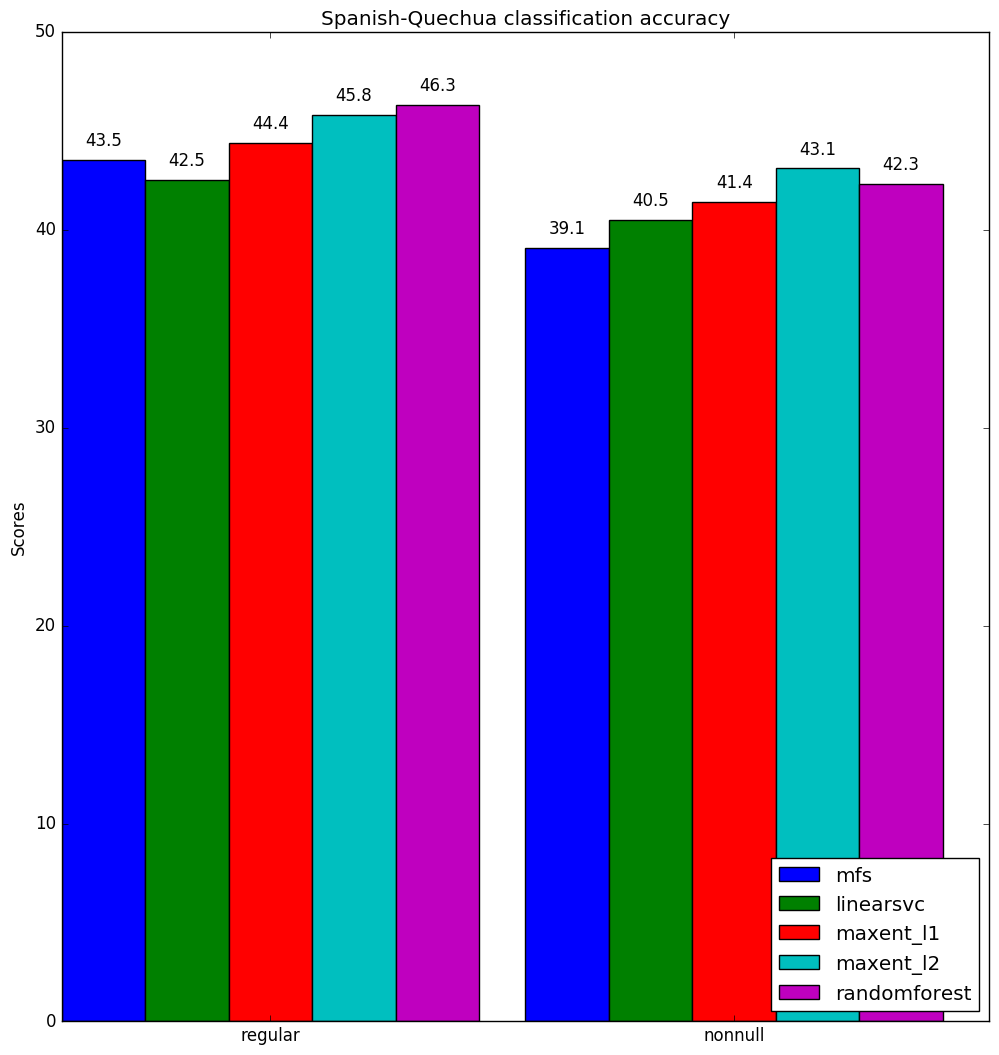
\includegraphics[width=\textwidth]{results-baseline-es-qu.png}
  \caption{Baseline Chipa scores for Spanish-Quechua, by classifier.}
  \label{fig:esquresults:baseline}
\end{figure}

\begin{figure}
  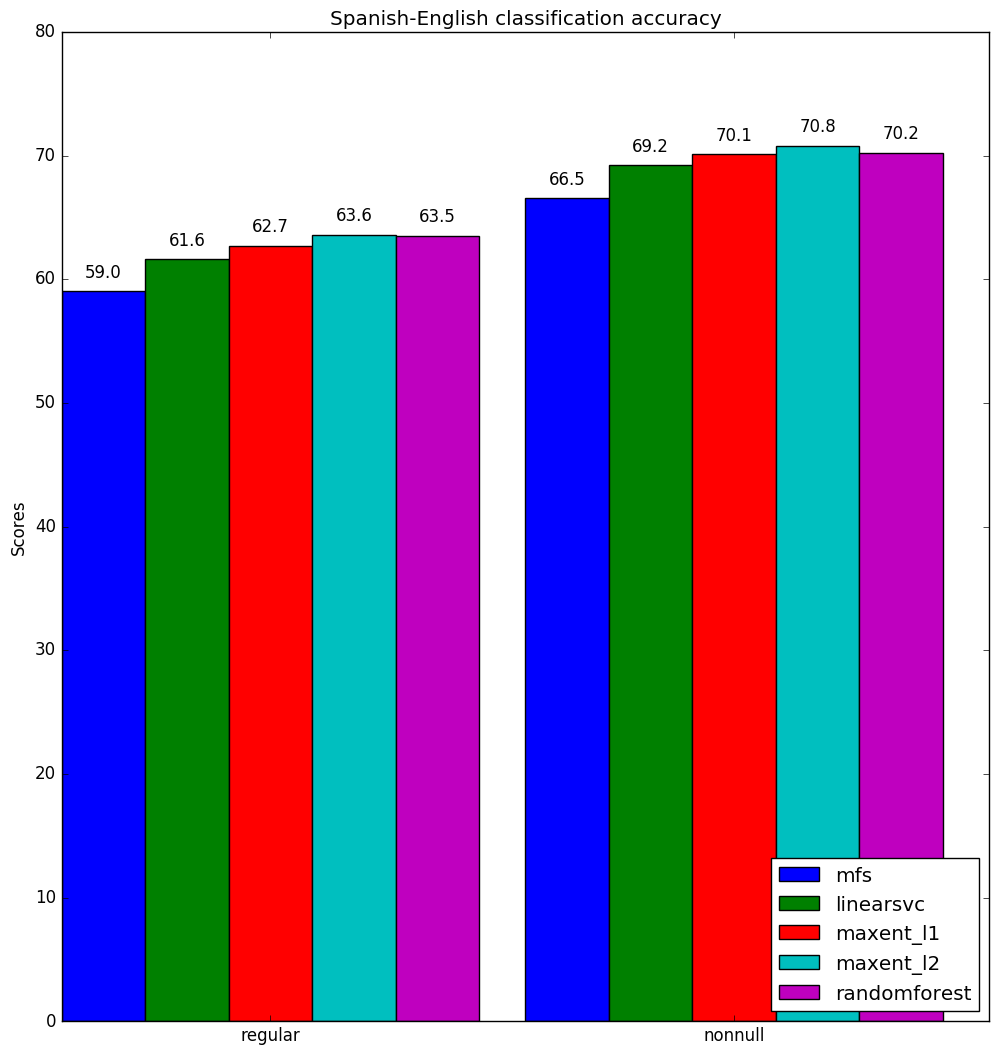
\includegraphics[width=\textwidth]{results-baseline-es-en.png}
  \caption{Baseline Chipa scores for Spanish-English, by classifier.}
  \label{fig:esenresults:baseline}
\end{figure}

\begin{figure}
  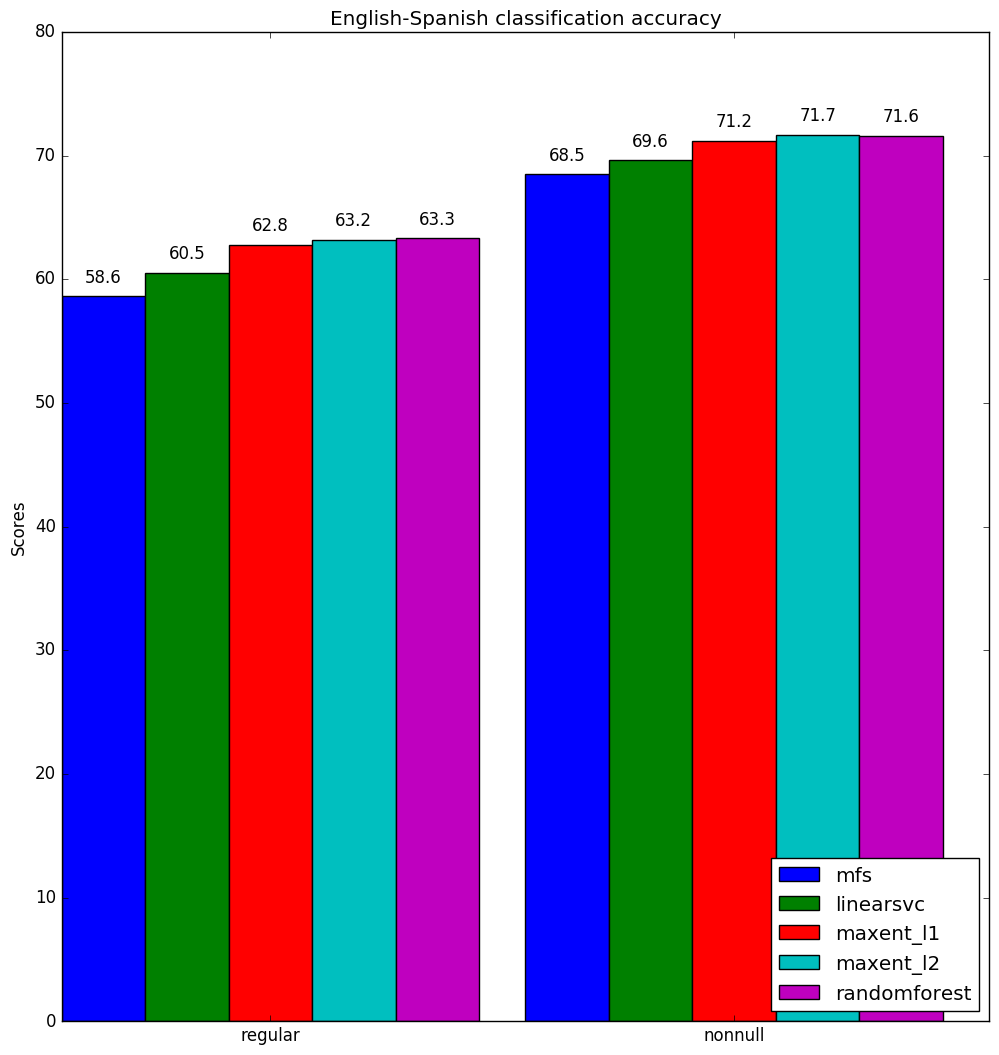
\includegraphics[width=\textwidth]{results-baseline-en-es.png}
  \caption{Baseline Chipa scores for English-Spanish, by classifier.}
  \label{fig:enesresults:baseline}
\end{figure}

In Figures \ref{fig:esgnresults:baseline}, \ref{fig:esquresults:baseline},
\ref{fig:esenresults:baseline}, and \ref{fig:enesresults:baseline}, we see the
results for the baseline Chipa system running with a a variety of common
classification algorithms, chosen for familiarity and availability within our
machine learning toolkit, on different language pairs. Here we report
classification accuracy as a percentage -- there is only one reference
translation given, and the classifier only gets credit for predicting it
correctly. We performed ten-fold cross-validation, using all of the available
training data for each of the lemmas in a given language pair's bitext that
appear at least fifty times. 

As mentioned previously, there are two settings for this task; in the
``regular" setting, we consider ``null" to be a valid translation, i.e., the
classifier must consider the possibility that the focus word is not explicitly
represented in the target-language sentence. In the ``nonnull" setting, we only
consider the instances where there is an alignment from the focus word to at
least one token in the target sentence. For most of the language pairs, we see
that our results in the ``nonnull" setting are higher, which is not surprising,
since there are fewer options to pick from. In Spanish-Quechua (Figure
\ref{fig:esquresults:baseline}), however, we see
that the scores are lower in the ``nonnull" setting. This seems to be due to
the Spanish and Quechua texts not being close translations of one another -- it
is fairly likely that words in the Spanish text are simply not present in the
Quechua text, so when this possibility is eliminated, the classifier must make
a more difficult choice from among the remaining options.

In nearly all of the settings for this task, the use of a classifier
outperformed the most-frequent sense baseline. We see a little variety in the
top results, for the four different language pairs and both task settings, but
the most successful classifiers here seem to be the maximum entropy classifier
with L2 regularization and random forests. The other classifiers post slightly
worse performance, but nearly always beat the MFS baseline.

So far, with commonly-used classifiers trained on commonly-used features, we
achieve a substantial boost on our ability to translate common polysemous words
from Spanish into two under-resourced languages, as well as between English and
Spanish, over a simple baseline. In subsequent chapters, we will see how to
build on this simple approach, largely through making additional features
available to the learning algorithms.

\section{For Comparison: the Baseline Chipa System On the SemEval 2010 and 2013
Shared Tasks}
\label{sec:baseline-semeval}

In order to situate this baseline Chipa system among other recent approaches to
CL-WSD, we ran Chipa on the SemEval CL-WSD test sets from 2010 and 2013, for
English-Spanish.
In the full 2010 and 2013 tasks, systems were also asked to translate into four
other European languages: German, Dutch, French and Italian. 
Here for simplicity, we focus on English-Spanish, since Chipa's preprocessing
pipeline already handles these languages, and the results across language pairs
were not drastically different in the original shared tasks.
In this task, we are presented with sentences in English, with a particular
focus word marked, and the goal is to select the lemma of a contextually
appropriate translation for that word\cite{lefever-hoste:2010:SemEval,task10}.
The task here guarantees that the appropriate translations are only those
present in the Europarl bitext, and several possible gold-standard translations
are provided by human annotators.  We made no particular additional effort to
tune Chipa for these tasks -- it was run here with the same settings used for
the Spanish-Guarani and Spanish-Quechua CL-WSD tasks, although the Chipa
codebase is descended from a system originally built for the 2013 task
\cite{rudnick-liu-gasser:2013:SemEval-2013}.

The training data for this task is considerably larger than the Bible text used
for the main CL-WSD task described in this work; Europarl bitext corpora
contain nearly 2 million parallel sentences. We applied the preprocessing steps
described in Section \ref{sec:datasetsandpreprocessing} to the Europarl bitext,
with the simplification that the individual sentences need not be extracted
from the various distribution formats used for Bibles.
Here we use only a very small modification to the Chipa system in order to
address the larger training data size; rather than holding the entire corpus in
memory, the corpus is kept on disk and scanned for sentences that contain the
current focus word before we need to train the CL-WSD classifier for a given
lemma.

\begin{figure}
  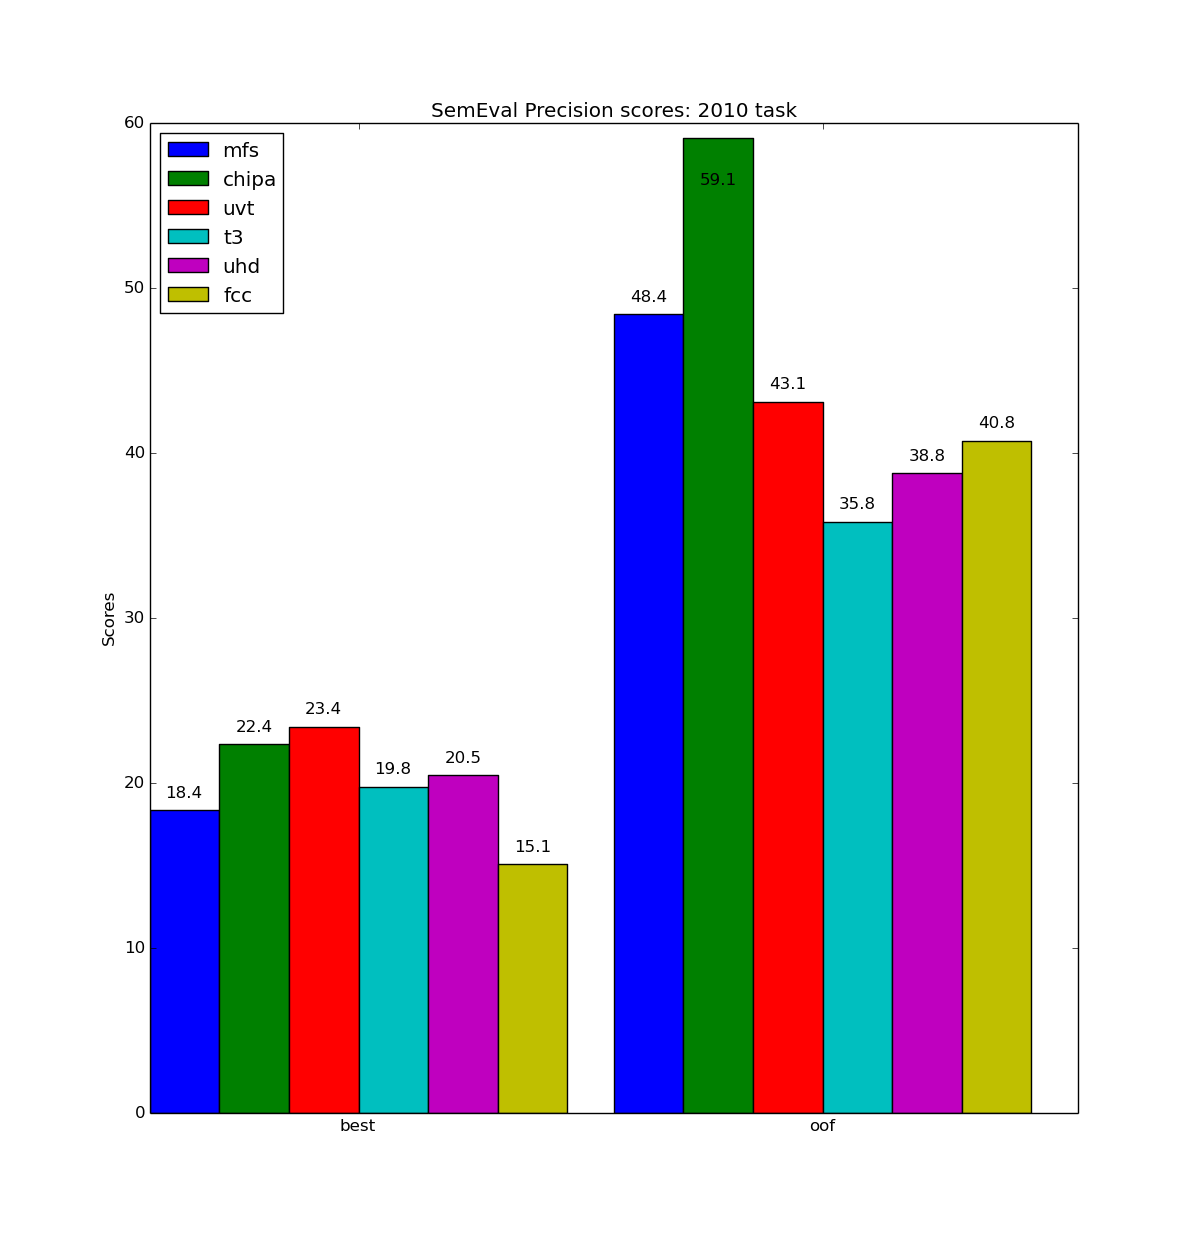
\includegraphics[width=\textwidth]{semeval-2010-ch4.png}
  \caption{Scores on the SemEval 2010 test set, including results posted in
  the shared task and the baseline Chipa system running on the same test set.}
  \label{fig:semeval2010:baseline}
\end{figure}

\begin{figure}
  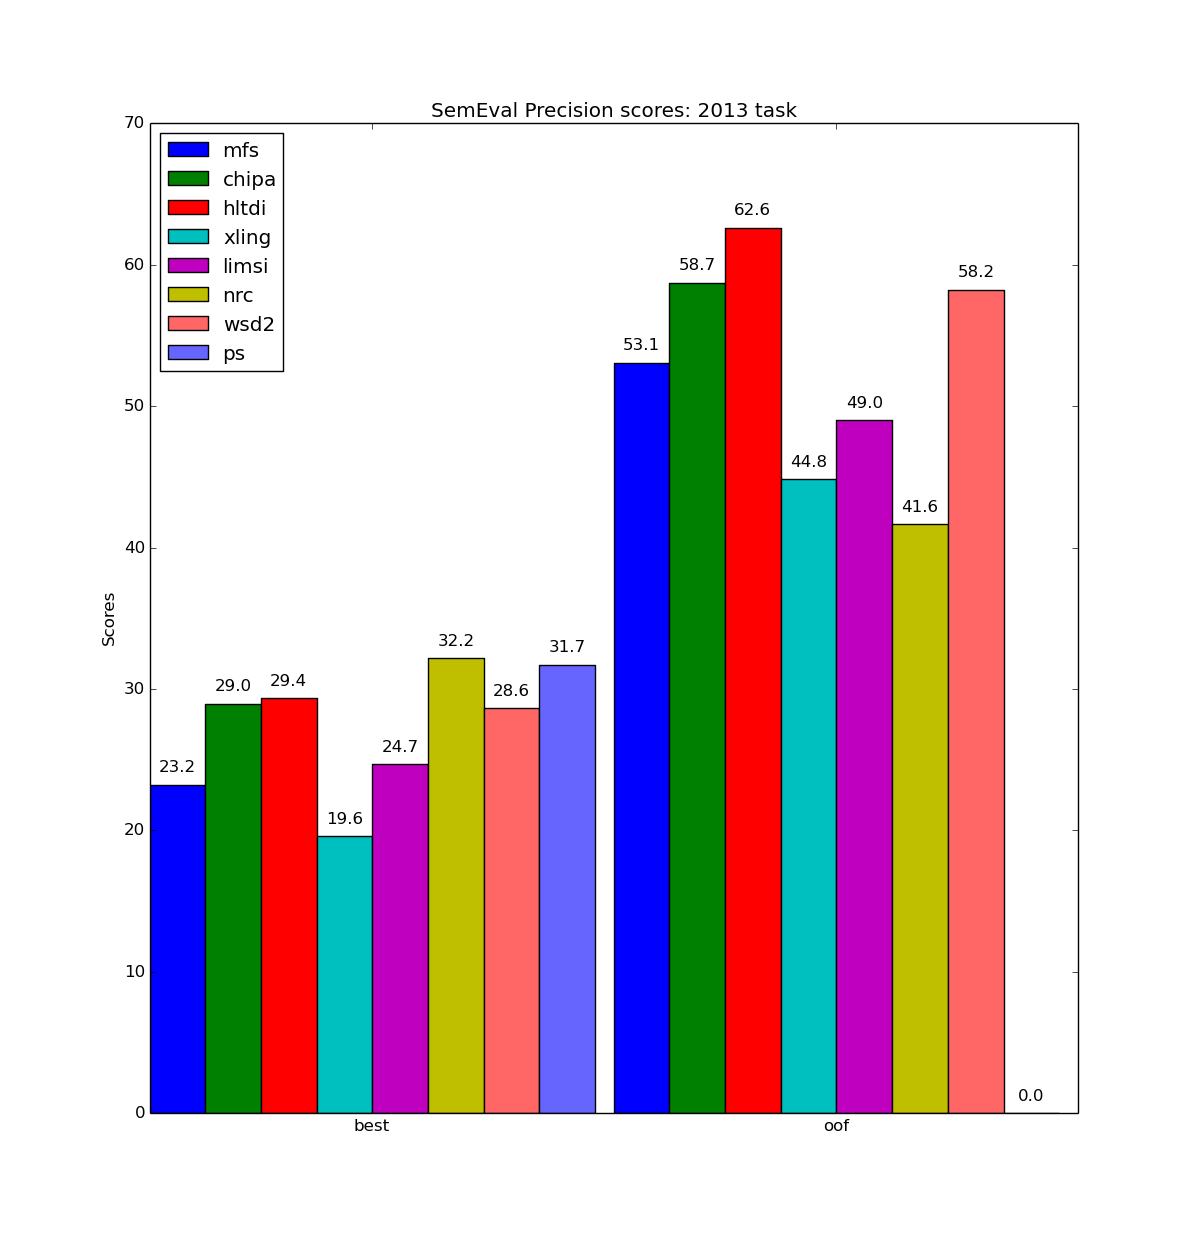
\includegraphics[width=\textwidth]{semeval-2013-ch4.png}
  \caption{Scores on the SemEval 2013 test set, including results posted in
  the shared task and the baseline Chipa system running on the same test set.
  When one team presented multiple results, here we take the best result from
  that team.}
  \label{fig:semeval2013:baseline}
\end{figure}

There were two settings for the evaluation, \emph{best} and \emph{oof}. In
either case, systems may present multiple possible answers for a given
translation, although in the \emph{best} setting, the first answer is given
more weight in the evaluation, and the scoring encourages only returning the
top answer.
In the \emph{oof} setting, systems are asked to return the top-five most likely
translations. In both settings, the answers are compared against translations
provided by several human annotators for each test sentence, who provided a
number of possible target-language translations in lemmatized form.  More
points are given for matching the more popular translations given by the
annotators. For a complete explanation of the evaluation and its scoring,
please see the shared task descriptions.

The scores for the baseline Chipa system, as well as for other systems
entered in the 2010 and 2013 competitions, are reported in Figures
\ref{fig:semeval2010:baseline} and \ref{fig:semeval2013:baseline}.
In the 2010 competition, none of the posted systems were able to beat the
simple most-frequent-sense baseline for the out-of-five setting, but Chipa
surpasses it handily. Chipa also does better than all but one of the posted
systems in the one-best setting. On the 2013 test set, Chipa also did fairly
well, scoring better than several of the posted systems in the one-best
setting, and all but one of the posted systems in the best-of-five. 
It should be noted that in the 2013 competitions, one of the posted systems
showing higher scores than the Chipa baseline was ``HLTDI", developed by myself
and Can Liu\cite{rudnick-liu-gasser:2013:SemEval-2013}, which made use of early
versions of some of the techniques described in subsequent chapters.

But we see here that this straightforward approach, using a maximum entropy
classifier with features extracted from the words and lemmas surrounding the
focus word, works quite well compared with the other systems in the shared
task, and so I claim that this is a sensible baseline on top of which we can
build more advanced approaches.
